% classes
\documentclass{article}

% packages
\usepackage{graphicx}
\usepackage{fancyhdr} % Required for custom headers
\usepackage{lastpage} % Required to determine the last page for the footer
\usepackage{extramarks} % Required for headers and footers
\usepackage{courier} % Required for the courier font

\usepackage{color}
\usepackage{enumitem}

\usepackage{hyperref}

\usepackage{fancyvrb}
\newenvironment{Schunk}{}{}
\DefineVerbatimEnvironment{Sinput}{Verbatim}{fontshape=sl}

\newcommand{\code}[1]{\texttt{#1}}
% \newcommand{\pkg}[1]{\mbox{\textbf{#1}}}
\newcommand{\pkg}[1]{\mbox{\texttt{#1}}}
\newcommand{\proglang}[1]{\textsf{#1}}

\usepackage[T1]{fontenc}

% page layout

\topmargin=-0.45in
\evensidemargin=0in
\oddsidemargin=0in

\textwidth=6.5in
\textheight=9.0in

\headsep=0.25in

\linespread{1.1} % Line spacing
 
\pagestyle{fancy}

% headers and footers

\fancyhf{}

\lhead{INTR 100 Breaking Intuition}

\rhead{
\includegraphics[width=0.045\textwidth]{wmlogo.jpg}}

\cfoot{Page \thepage}


% document body

\begin{document}

\vspace*{.01mm}

\begin{center}

\Large{\textcolor{blue}{\textbf{Introductory Lab.}  A Gentle Introduction to Data}}

\vspace{4mm}

\textit{Due by noon on Friday, August 28th}\\

\end{center}

\begin{figure}[h!]
\begin{center}
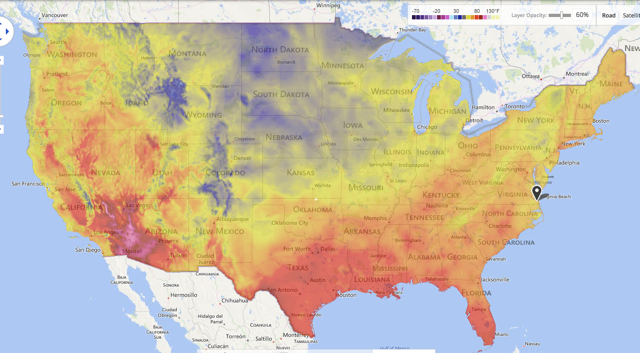
\includegraphics[width=1.0\textwidth]{weather.png}

\end{center}
\end{figure}

\setlength{\parindent}{0cm}

\large{\textit{"Everything is related to everything else, but near things are more related than distant things."}
\begin{flushright}
Tobler, 1970
\end{flushright}
}




\newpage

% Enumerate the Laboratory Objectives

\large{\textbf{Laboratory in Brief:}}

\vspace{4mm}

\setlength{\leftskip}{1cm}

\setlength{\parindent}{0cm}

The purpose of this laboratory is to introduce you to \textit{the world of tomorrow}.  More directly, you'll be learning a few of the fundamentals you'll need later in the course.  This is \textbf{NOT} a programming course (I promise!), but you'll need to at least be able to type a few things in here and there that may - deceptively - look a little bit like programming.  To get you started off, we're going to very, very slowly introduce you to a few concepts used in the statistical language \textit{R}.

\vspace{4mm}

\setlength{\leftskip}{0cm}

\large{\textbf{Goals of this Laboratory:}}

\begin{enumerate}[leftmargin=15mm]

\item To learn how to install and load "packages" - magic tools other people have written that will let us do incredible things.

\item To learn how to make a map using \textit{R}!  You'll be the envy of your friends.

\end{enumerate}

% Enumerate the Laboratory Resources Needed

%\large{\textbf{Things to do in Preparation for this Lab:}}

%\begin{enumerate}[leftmargin=15mm]

%\item ...

%\item ...

%\item ...

%\end{enumerate}

% Step by Step Instructions for Day 1

\large{\textbf{Session 1: Wednesday, August 26th}}

\vspace{4mm}
\setlength{\leftskip}{1cm}
\textit{Acquire all the Data!} {\tiny Kind of...}

\begin{enumerate}[leftmargin=15mm]

\item First lets open \proglang{RStudio}.  You'll find it as a link in your start menu (if you're really brave, you could even install this at home!).

\item One of the most basic features of R is a package.  A package is an external source of code that can be installed into your local system that has specific features for executing a particular function.  

\item Using a package is a two-step process.  First, just like any other app, you need to install.  Second, you need to "load" it inside of RStudio (just like you have to launch an app every time you use it).

\item Installing the package only needs to be done one time, while loading it needs to be done each time we want to use it in \proglang{R}.  To do this first we install the package by typing the following command:

\begin{Schunk}
\begin{Sinput}
install.packages("ggmap", dependencies=TRUE)
\end{Sinput}
\end{Schunk}

This particular package, ggmap, will let us make our map!  Adding the command \code{dependencies=TRUE} tells \proglang{R} to install all the other applications \pkg{ggmap} needs to function properly.  You don't \textit{always} need this, but better safe than sorry.

\item Once you have installed the package \pkg{ggmap}, next you will need to load it into \proglang{R}. To do this type the following command (and then, if you haven't figured it out yet, hit enter).

\begin{Schunk}
\begin{Sinput}
library(ggmap)
\end{Sinput}
\end{Schunk}

and your package is now active and ready for use.

\item I know that was exciting, but now we're headed to the \textit{really} fun part. Just like a word document, you can save all the things you do in R.  To do this, lets create a new file (File -> New File -> R Script).  Now, click file -> Save.  Choose your H drive and save it as something you'll remember later!

\item Now it's time to get coding.  Let's go \textit{CRAZY}, and type the following into our new document (R Script): 

\begin{Schunk}
\begin{Sinput}
1 + 1
\end{Sinput}
\end{Schunk}

Highlight that entire thing (yes, ALL of 1+1), and then click the 'run' button in the upper-right hand corner.  Just like that, we've tricked you into becoming a programmer.

\item Now, lets make a "quick map" in R by assigning a place to a variable. Since we are going to create a map of our favourite University, I will use one of my favourite places.

\begin{Schunk}
\begin{Sinput}
gt = 'Georgia Tech'
\end{Sinput}
\end{Schunk}

To understand what we have done, simply type \code{ gt} and have a look at the output from \proglang{R}.

\item Now lets execute our first function in \proglang{R}.  The package \pkg{ggmap} has a quick map function that takes a name and attempts to figure out what you are interested in mapping, and then creates a map for you.  To make this work, your R document should look like the below:

\begin{Schunk}
\begin{Sinput}
library(ggmap)
gt = 'Georgia Tech'
qmap(gt, zoom = 14)
\end{Sinput}
\end{Schunk}

We can also play around with the qmap function by adding some other commands, known as "arguments".  Run the below three examples one at a time to see how this can work.

\begin{Schunk}
\begin{Sinput}

Example 1: qmap(gt, zoom = 13, source = "osm")

Example 2: qmap(gt, zoom = 15, source = "stamen", 
maptype = "watercolor", crop = FALSE)

Example 3: qmap(gt, zoom = 16, source = "stamen", 
maptype = "toner", crop = FALSE)

\end{Sinput}
\end{Schunk}

\item \textbf{\textit{Deliverable Number 1:  Create a map of your home town, favourite school, or university, and copy it into a word document - full points will be awarded for using a different type of map source or map type.}}

\item NOTE: The help pages in \proglang{R} are notoriously difficult to read, but once you get the hang of them, they can be informative.  In order to find out more information about a particular function type \code{?qmap} and the help page for that function will pop up.


\item Next we will use the \code{get\_map} function in \pkg{ggmap}.  This function works similar to the qmap function, but now we will be able to have more control over the output.  Type the following command.

\begin{Schunk}
\begin{Sinput}

santos = get_map(location = "Santos", zoom = 12)

\end{Sinput}
\end{Schunk}

\item Here, we have created an object called 'santos' in \proglang{R}.  One important convention to understand, is when \proglang{R} programmers refer to a function, they generally refer to it with two parentheses after the function name, for example \code{get\_map()}.  You can type the name of the object \code{santos} into the \proglang{R} console, but this isn't going to be very helpful, since it will just print the data within the object.  You can look at it and see it it makes any sense to you.  Once you are finished lets use the \code{ggmap()} command to print our map of Santos, Brazil.

\item Did you just type in ggmap and get an error?  Caught you!  ggmap() is a \textit{function}, as you can see by the () after the word "ggmap".  Many functions require more information before they'll work - in this case, you need the information we saved into "santos" earlier.  Try this:

\begin{Schunk}
\begin{Sinput}

ggmap(santos)

\end{Sinput}
\end{Schunk}

We can begin to do more with the \pkg{ggmap} package like add labels for the X and Y axis as well as give our plot a title.

\begin{Schunk}
\begin{Sinput}

ggmap(santos) + labs(x = 'Longitude', y = 'Latitude') 
+ ggtitle('The Home of Pele')

\end{Sinput}
\end{Schunk}

\item As before, in order to find out more information about a particular function type \code{?ggmap} and the help page for that function will pop up.

\item \textbf{\textit{Deliverable Number 2:  Now create a map of a place you would like to visit one day, and copy it into your word document.  Make something that is visually interesting to you!}}


\vspace{4mm}
\setlength{\leftskip}{1cm}
\newpage
\large{\textbf{Final Output for Submission}}\\
That's it!  This assignment will be turned in for a grade, and is 
\textit{due by 11:59PM EST on Friday, August 28th - note, Blackboard will NOT accept submissions after this deadline!:}

\vspace{2mm}

Make certain the word document you turn in on blackboard has the following:

\begin{itemize}

\item Your name!
\item A Map of your favourite School, University, or home town.
\item A Map of a place you would like to visit one day
\item A copy of the code you used to produce each of the above maps.
\item Any stretch goals you choose to include (see the next page).

\end{itemize}

There are few wrong answers to most labs in this course, but creativity is heavily encouraged to reach the highest grades.  Make your visuals look good, use your data to make compelling arguments, and don't worry about "getting it wrong"!  



\newpage 
{\huge Stretch Goals}\\
Most labs in this course will have "stretch goals" - challenges that can be turned in for extra credit on your lab (note your grade cannot exceed 100!).  These goals are designed to be more difficult than the mandatory assignment, and may require more critical thinking (or, even googling!) to solve.  Good luck, and never hesitate to come talk with a TA or professor!


\item Next, we will import a shape file and do some very basic spatial statistics on it.  To start lets install and load the \pkg{rgdal} just as we installed and loaded \pkg{ggmap}.

\begin{Schunk}
\begin{Sinput}
install.packages("rgdal", dependencies=TRUE)
library(rgdal)
\end{Sinput}
\end{Schunk}

We will also want to use a new \proglang{R} command in order to set the working directory.  The working directory is the location where \proglang{R} will look for files that are being referenced as part of a command.  While we can always specify the full path for a file, its often just easier to set the working directory in order to prevent our programming from becoming to verbose.  For example (note, you'll need to change this working directory path to where YOU have the lab downloaded.  This part may be hard if you've never done it before, so don't hesitate to ask for help from a TA or professor!).

\begin{Schunk}
\begin{Sinput}
setwd("/Users/tyfrazier/workspace/work_life/WM/Teaching/
COLL_100/labs/lab1_basics")
\end{Sinput}
\end{Schunk}

\item Now lets read a shape file into \proglang{R} and create a new "spatial object".  A shapefile is essentially a file that defines the lines of a map.  We use the \code{readOGR()} function in order to accomplish this task.  The \code{readOGR()} function takes two qualifiers the \code{den =} specifier and the \code{layer =} specifier.  The \code{dsn = } is just the name of the folder where the shape file and its supporting files are located.  The \code{layer =} qualifier is just the name of the shape file. 

\begin{Schunk}
\begin{Sinput}
acr = readOGR(dsn = "data", layer = "accra")
\end{Sinput}
\end{Schunk}

This function will import the shape file named accra and create the \proglang{R} object named \code{acr}, which is simply a shortened naming convention for the capital city of Ghana.

\item Finally, we will use the \pkg{tmap} to print a few basic spatial maps that describe Accra.  Again lets install and load the package.

\begin{Schunk}
\begin{Sinput}
install.packages("tmap", dependencies=TRUE)
library(tmap)
\end{Sinput}
\end{Schunk}

Now we will use the \code{qtm()} function to spatially describe a variable.  One variable we can use is named \code{SLUM\_INDEX}.  So lets use it.

\begin{Schunk}
\begin{Sinput}
qtm(shp = acr, fill = "SLUM_INDEX", 
fill.palette = "-Blues")
\end{Sinput}
\end{Schunk}

We can also plot two variables side by side and compare them.  Another variable we can use gives us the number of households per enumeration area.

\begin{Schunk}
\begin{Sinput}
qtm(shp = acr, fill = c("SLUM_INDEX", "N_HH_POP"), 
fill.palette = c("Blues"), ncol = 2)
\end{Sinput}
\end{Schunk}



\item \textbf{\textit{Stretch Deliverable: Copy your variables in a side-by-side comparison, and show the code you used to produce them. }}
\end{enumerate}

% Final Output from Laboratory

\setlength{\leftskip}{0cm}





% Grading

\setlength{\leftskip}{0cm}


%----------------------------------------------------------------------------------------

\end{document}